\chapter{Training Observables for $K_S^0$ Classifier}

\begin{figure}[H]
	\caption{The distribution of Ks training variables. The red is the from fake $K_S^0$ and the blue is from true $K_S^0$}
\begin{subfigure}{0.5\linewidth}
	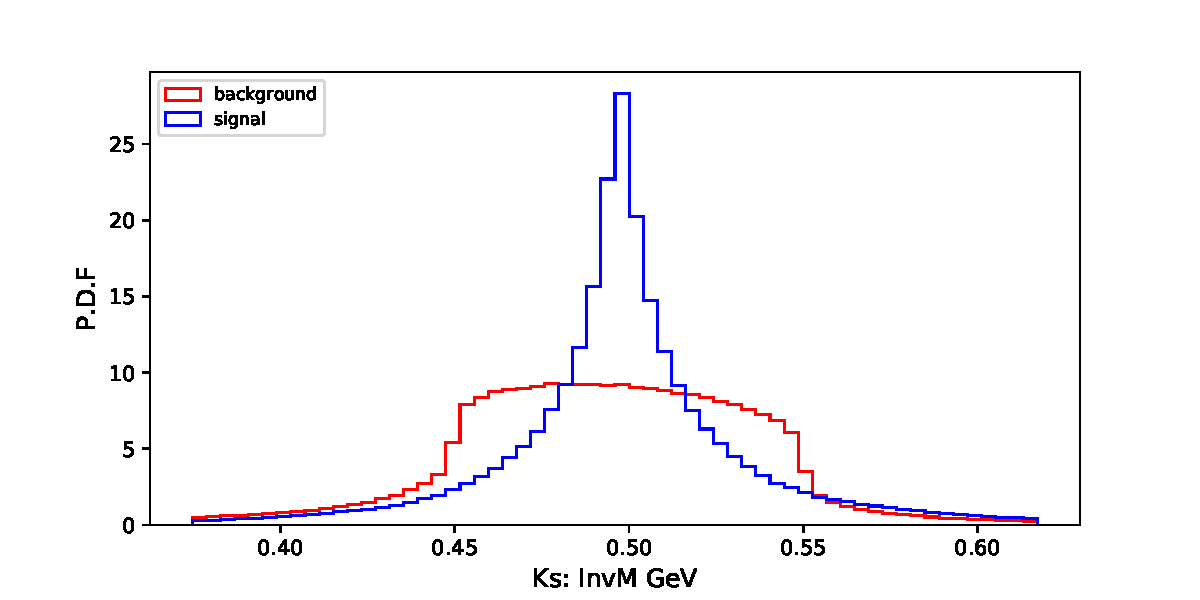
\includegraphics[page=1,height=4cm]{FastBDT_eval.pdf}
\end{subfigure}
\begin{subfigure}{0.5\linewidth}
		\includegraphics[page=2,height=4cm]{FastBDT_eval.pdf}
\end{subfigure}
\begin{subfigure}{0.5\linewidth}
		\includegraphics[page=3,height=4cm]{FastBDT_eval.pdf}
\end{subfigure}
\begin{subfigure}{0.5\linewidth}
		\includegraphics[page=4,height=4cm]{FastBDT_eval.pdf}
\end{subfigure}
\begin{subfigure}{0.5\linewidth}
		\includegraphics[page=5,height=4cm]{FastBDT_eval.pdf}
\end{subfigure}
\begin{subfigure}{0.5\linewidth}
	\includegraphics[page=6,height=4cm]{FastBDT_eval.pdf}
\end{subfigure}
\end{figure}

\begin{figure}[H]
\ContinuedFloat
\begin{subfigure}{0.5\linewidth}
	\includegraphics[page=7,height=4cm]{FastBDT_eval.pdf}
\end{subfigure}
\begin{subfigure}{0.5\linewidth}
	\includegraphics[page=8,height=4cm]{FastBDT_eval.pdf}
\end{subfigure}
\begin{subfigure}{0.5\linewidth}
	\includegraphics[page=9,height=4cm]{FastBDT_eval.pdf}
\end{subfigure}
\begin{subfigure}{0.5\linewidth}
	\includegraphics[page=10,height=4cm]{FastBDT_eval.pdf}
\end{subfigure}
\begin{subfigure}{0.5\linewidth}
	\includegraphics[page=11,height=4cm]{FastBDT_eval.pdf}
\end{subfigure}
\begin{subfigure}{0.5\linewidth}
	\includegraphics[page=12,height=4cm]{FastBDT_eval.pdf}
\end{subfigure}
\begin{subfigure}{0.5\linewidth}
	\includegraphics[page=13,height=4cm]{FastBDT_eval.pdf}
\end{subfigure}
\begin{subfigure}{0.5\linewidth}
	\includegraphics[page=14,height=4cm]{FastBDT_eval.pdf}
\end{subfigure}
\begin{subfigure}{0.5\linewidth}
	\includegraphics[page=15,height=4cm]{FastBDT_eval.pdf}
\end{subfigure}
\begin{subfigure}{0.5\linewidth}
	\includegraphics[page=16,height=4cm]{FastBDT_eval.pdf}
\end{subfigure}
\end{figure}

\begin{figure}[H]
\begin{subfigure}{0.5\linewidth}
	\includegraphics[page=17,height=4cm]{FastBDT_eval.pdf}
\end{subfigure}
\begin{subfigure}{0.5\linewidth}
	\includegraphics[page=18,height=4cm]{FastBDT_eval.pdf}
\end{subfigure}
\begin{subfigure}{0.5\linewidth}
	\includegraphics[page=19,height=4cm]{FastBDT_eval.pdf}
\end{subfigure}
\begin{subfigure}{0.5\linewidth}
	\includegraphics[page=22,height=4cm]{FastBDT_eval.pdf}
\end{subfigure}
\begin{subfigure}{0.5\linewidth}
	\includegraphics[page=23,height=4cm]{FastBDT_eval.pdf}
\end{subfigure}
\begin{subfigure}{0.5\linewidth}
	\includegraphics[page=24,height=4cm]{FastBDT_eval.pdf}
\end{subfigure}
\begin{subfigure}{0.5\linewidth}
	\includegraphics[page=25,height=4cm]{FastBDT_eval.pdf}
\end{subfigure}
\begin{subfigure}{0.5\linewidth}
	\includegraphics[page=26,height=4cm]{FastBDT_eval.pdf}
\end{subfigure}
\begin{subfigure}{0.5\linewidth}
	\includegraphics[page=27,height=4cm]{FastBDT_eval.pdf}
\end{subfigure}
	
\end{figure}


\clearpage
\newpage